\documentclass[10pt]{article}
\usepackage[paperwidth=42cm,paperheight=64.2cm,margin=1.2cm]{geometry}
\usepackage{amsmath,amssymb}
\usepackage[T1]{fontenc}
\usepackage[scaled=0.92]{helvet}
\renewcommand{\familydefault}{\sfdefault}
\usepackage[table]{xcolor}
\usepackage[most]{tcolorbox}
\usepackage{tikz}
\usetikzlibrary{arrows.meta,calc,shapes.geometric}
\usepackage{array}
\pagestyle{empty}
\setlength{\parindent}{0pt}
\setlength{\parskip}{5pt}
\renewcommand{\arraystretch}{1.35}

% ---------- colours ----------
\definecolor{cNavy}{HTML}{2B3A8F}
\definecolor{cGreen}{HTML}{2E8B57}
\definecolor{cGold}{HTML}{C9900C}
\definecolor{cSlate}{HTML}{3C4650}
\definecolor{cOrange}{HTML}{E0701A}
\definecolor{cRed}{HTML}{C8323C}
\definecolor{cTeal}{HTML}{14857A}
\definecolor{cBlue}{HTML}{2F4FA8}
\definecolor{cPurple}{HTML}{6A3FA0}
\definecolor{cMagenta}{HTML}{B0306A}
\definecolor{cGray}{HTML}{6B6B6B}

% ---------- notation ----------
\newcommand{\R}{\mathbb{R}}
\newcommand{\cO}{\mathcal{O}}
\newcommand{\cT}{\mathcal{T}}
\newcommand{\cB}{\mathcal{B}}

% ---------- boxes ----------
\newcommand{\badge}[2]{\tikz[baseline=(b.base)]\node[circle,fill=#1,text=white,inner sep=0pt,
  minimum size=1.55em,font=\sffamily\bfseries\Large](b){#2};}
\newtcolorbox{panel}[3]{enhanced,colback=white,colframe=#1,boxrule=1.5pt,arc=3mm,
  title={\badge{#1}{#2}\hspace{0.45em}#3},coltitle=#1,colbacktitle=white,
  fonttitle=\sffamily\bfseries\LARGE,titlerule=0pt,toptitle=2.5mm,bottomtitle=0mm,
  left=3.5mm,right=3.5mm,top=1mm,bottom=2.5mm,before skip=0pt,after skip=6mm}
\newtcolorbox{keybox}[1][cNavy]{enhanced,colback=#1!6,colframe=#1!70,boxrule=0.8pt,arc=2mm,
  left=2.5mm,right=2.5mm,top=1mm,bottom=1mm,before skip=4pt,after skip=5pt}
\newtcolorbox{rowbox}{enhanced,sidebyside,lefthand width=2.1cm,sidebyside align=center,
  segmentation hidden,colback=cGold!6,colframe=cGold!55,boxrule=0.7pt,arc=1.5mm,
  left=2mm,right=2mm,top=1.5mm,bottom=1.5mm,before skip=3pt,after skip=4pt}
\newcommand{\lab}[2]{\textbf{\color{#1}#2}}
\newcommand{\remk}[2]{{\color{#1}\itshape #2}}

% ---------- pictures ----------
\newcommand{\sectorpic}[1]{%
\begin{tikzpicture}[scale=#1]
  \fill[cOrange!45] (0,0) circle (1);
  \fill[white] (0,0) circle (0.5);
  \foreach \a in {0,180}{
    \fill[cBlue!50] (\a-17:0.5) arc[start angle=\a-17,end angle=\a+17,radius=0.5]
      -- (\a+17:1) arc[start angle=\a+17,end angle=\a-17,radius=1] -- cycle;
    \fill[gray!35] (\a+17:0.5) arc[start angle=\a+17,end angle=\a+24,radius=0.5]
      -- (\a+24:1) arc[start angle=\a+24,end angle=\a+17,radius=1] -- cycle;
    \fill[gray!35] (\a-24:0.5) arc[start angle=\a-24,end angle=\a-17,radius=0.5]
      -- (\a-17:1) arc[start angle=\a-17,end angle=\a-24,radius=1] -- cycle;}
  \draw[-{Stealth}] (-1.25,0)--(1.3,0) node[right]{$\xi_1$};
  \draw[-{Stealth}] (0,-1.25)--(0,1.3) node[above]{$\xi_2$};
\end{tikzpicture}}

\newsavebox{\colbox}
\begin{document}

% ================= HEADER =================
\begin{center}
{\fontsize{44}{52}\selectfont\bfseries\color{cNavy}Sector decomposition for an anisotropic phase\par}
\vspace{5mm}
{\LARGE\itshape\color{cGray}A stationary phase bound, sector by sector and uniformly in $x$, for
$\displaystyle I(t,x)=\int_{\R^d}e^{i(x\cdot\xi-\psi(t,\xi))}\,|A_t\xi|^{-1}\chi(\xi)\,d\xi$.\par
\vspace{1mm}
Every symbol is defined on this sheet, and every step comes with its reason.\par}
\end{center}
\vspace{6mm}

% ================= COLUMN 1 =================
\noindent
\begin{minipage}[t]{0.322\textwidth}\vspace{0pt}

\begin{panel}{cNavy}{A}{THE PROBLEM}
Fix exponents $\ell_1,\dots,\ell_d\ge0$ and, for $s>0$, let
$A_s=\operatorname{diag}(s^{\ell_1},\dots,s^{\ell_d})$. A wave moves with speed $s^{\ell_j}$
in direction $j$, so after time $t$ it carries the phase
\[
\psi(t,\xi)=\int_1^t|A_s\xi|\,ds .
\]
For $t\ge2$ and $x\in\R^d$ we study
\begin{keybox}[cNavy]
\[
I(t,x)=\int_{\R^d}e^{i(x\cdot\xi-\psi(t,\xi))}\,|A_t\xi|^{-1}\,\chi(\xi)\,d\xi ,
\]
\end{keybox}
where $\chi$ is smooth and supported in $\tfrac12\le|\xi|\le2$.

\lab{cNavy}{Goal.} Bound $\sup_x|I(t,x)|$ for large $t$, one sector at a time.

\lab{cNavy}{Directions seen from sector $k$.} For $j\ne k$ put
\[
\kappa_j=2\ell_j-\ell_k+1 .
\]
Direction $j$ is \emph{good} if $\ell_j\ge\ell_k$ and \emph{bad} if $\ell_j<\ell_k$.
It is \emph{oscillatory} if $\kappa_j>0$ and \emph{non-oscillatory} if $\kappa_j\le0$.
\begin{itemize}\setlength{\itemsep}{1pt}
  \item $\cO$: oscillatory directions. Every good direction is in $\cO$, since $\kappa_j\ge\ell_k+1>0$.
  \item $\cT$: non-oscillatory directions. They are all bad.
  \item $\cB=\cO\cap\{\text{bad}\}$: bad oscillatory directions.
\end{itemize}
\end{panel}

\begin{panel}{cGreen}{B}{THE RESULT}
\begin{keybox}[cGreen]
\lab{cGreen}{Theorem (main estimate).} There are $t_0$ and $C$, depending only on $d$ and the
$\ell_j$, such that for $t\ge t_0$, all $x$ and all $\xi_k\ne0$,
\[
\Big|\int_{\R^{d-1}}e^{i\lambda\Phi(\eta)}\,b(\xi_k,\eta)\,d\eta\Big|
\le C\,\lambda^{-\frac{d-1}{2}}\prod_{j\in\cT}t^{\kappa_j/2}\,|\xi_k|^{-1/2},
\]
with $\lambda=t^{\ell_k+1}|\xi_k|$.
\end{keybox}
Here $\eta$, $\Phi$ and $b$ are the variables, phase and amplitude of the inner integral of
sector $k$ (Step 1).

\lab{cGreen}{Reading.} If $\cT$ is empty, this is the full stationary phase rate
$\lambda^{-(d-1)/2}$. Each factor from $\cT$ is at most $|\xi_k|^{-1/2}$.

\lab{cGreen}{Example.} $d=2$, $\ell_1=0$, $\ell_2=\ell>0$.

{\small
\begin{tabular}{@{}p{2.2cm}p{2.6cm}p{2.5cm}l@{}}
\textbf{\color{cGreen}sector} & \textbf{\color{cGreen}other direction} & \textbf{\color{cGreen}type} & \textbf{\color{cGreen}bound}\\\hline
$k=1$ & $j=2$, $\kappa=2\ell+1$ & good & $\lambda^{-1/2}\approx t^{-1/2}$\\
$k=2$, $\ell<1$ & $j=1$, $\kappa=1-\ell$ & bad, oscillatory & $(t^{\ell+1}|\xi_2|)^{-1/2}$\\
\rowcolor{cRed!10}$k=2$, $\ell\ge1$ & $j=1$, $\kappa=1-\ell$ & non-oscillatory & $t^{-\ell}|\xi_2|^{-1}$\\
\end{tabular}}

\remk{cGreen}{The outer $\xi_k$ integral, where $|\xi_k|$ can be as small as
$t^{\ell_{\min}-\ell_k}$, is not treated here.}
\end{panel}

\begin{panel}{cGold}{C}{WHY IT IS DELICATE}
\begin{rowbox}
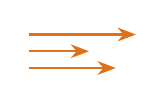
\begin{tikzpicture}[scale=0.85]
  \draw[-{Stealth},cOrange,thick] (0,0.5)--(1.6,0.5);
  \draw[-{Stealth},cOrange,thick] (0,0.25)--(0.9,0.25);
  \draw[-{Stealth},cOrange,thick] (0,0)--(1.3,0);
\end{tikzpicture}
\tcblower
Each direction has its own speed $s^{\ell_j}$. The phase is not radial, so no single large
parameter sits in front of it.
\end{rowbox}
\begin{rowbox}
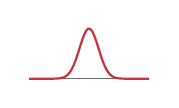
\begin{tikzpicture}[scale=0.85]
  \draw[cGray] (-0.9,0)--(0.9,0);
  \draw[cRed,thick,domain=-0.9:0.9,samples=60] plot (\x,{0.75*exp(-25*\x*\x)});
\end{tikzpicture}
\tcblower
In a bad direction, near $\eta_j=0$ the coordinate $j$ dominates at early times. High
derivatives of the phase then blow up as $t\to\infty$.
\end{rowbox}
\begin{rowbox}
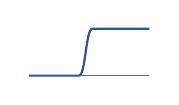
\begin{tikzpicture}[scale=0.85]
  \draw[cGray] (0,0)--(1.8,0);
  \draw[cBlue,thick] (0,0)--(0.75,0) .. controls (0.85,0) and (0.85,0.7) .. (0.95,0.7)--(1.8,0.7);
\end{tikzpicture}
\tcblower
Each $\partial_{\eta_j}$ on the cutoff costs $t^{\ell_k-\ell_j}$, which is huge for bad $j$.
A direct stationary phase bound loses $t^{d(\ell_k-\ell_{\min})}$.
\end{rowbox}
\end{panel}

\begin{panel}{cSlate}{0}{THE TOOL}
A stationary phase bound that does not see the size of the domain.
\begin{keybox}[cSlate]
\lab{cSlate}{Theorem 0 (Alazard, Burq, Zuily).} Let $b\in C_0^\infty(\R^n)$ have support $K$,
and let $K_1$ be the points at sup distance at most $1$ from $K$. Let $\Phi$ be real and
smooth near $K_1$, with
\[
a_0=\inf_{K_1}|\det\nabla^2\Phi|>0
\]
and $\nabla\Phi$ injective on $K_1$. Then for $\lambda\ge1$,
\[
\Big|\int e^{i\lambda\Phi}b\Big|\le\frac{C_n}{a_0}\,(1+M_{n+2})^{n/2}\,N_{n+1}\,\lambda^{-n/2},
\]
where $M_m=\sum_{2\le|\alpha|\le m}\sup_{K_1}|\partial^\alpha\Phi|$ and
$N_m=\sum_{|\alpha|\le m}\sup_K|\partial^\alpha b|$.
\end{keybox}
\lab{cSlate}{Why it fits.} No volume of $K$ appears, so a large support costs nothing.
$\Phi$ enters only through derivatives of order at least two, so the linear term that
carries $x$ is invisible.

{\footnotesize\color{cGray}T. Alazard, N. Burq, C. Zuily, \emph{A stationary phase type
estimate}, Proc.\ AMS 145 (2017), Theorem 3.}
\end{panel}


\begin{panel}{cSlate}{i}{NOTATION AT A GLANCE}
{\small
\begin{tabular}{@{}p{2.9cm}p{7.2cm}c@{}}
$k$, $\eta_j$, $\lambda$ & sector, chart ratios, large parameter $t^{\ell_k+1}|\xi_k|$ & 1\\
$G$, $H$, $\Phi$, $b$ & normal form, its integrand, inner phase, amplitude & 1\\
$\kappa_j$ & $2\ell_j-\ell_k+1$; its sign decides the type of direction $j$ & A\\
$\cO$, $\cT$, $\cB$ & oscillatory, non-oscillatory, bad oscillatory & A\\
$w_j$ & derivative weight: $1$ if good, $|\eta_j|$ if bad & 3\\
$\omega$, $\tilde\Phi$, $\tilde b$ & zoomed variable, phase, amplitude & 4\\
$\vartheta$, $S$, $A$, $W_j$ & strip cutoff, strip set, active set, width in $\cT$ & 5\\
\end{tabular}}
\end{panel}

\end{minipage}\hfill
% ================= COLUMN 2 =================
\begin{minipage}[t]{0.322\textwidth}\vspace{0pt}

\begin{panel}{cOrange}{1}{STEP 1 $\cdot$ SECTORS}
\begin{minipage}[c]{0.6\linewidth}
\lab{cOrange}{Sectors.} Sector $k$ is where $t^{\ell_k}|\xi_k|$ is the largest weight
$t^{\ell_j}|\xi_j|$. There $t^{\ell_k}|\xi_k|\ge|A_t\xi|/\sqrt d$.

\lab{cOrange}{Smooth sectors.} Take $\rho_k$ on $\mathbb S^{d-1}$ with $\sum_k\rho_k=1$ and
$\rho_k(\theta)=0$ unless $|\theta_k|\ge1/(2\sqrt d)$, and insert $\rho_k(A_t\xi/|A_t\xi|)$.
\end{minipage}\hfill
\begin{minipage}[c]{0.37\linewidth}\centering
\sectorpic{1.45}\\[1mm]
{\scriptsize $d=2$, $\ell_1<\ell_2$.\\
\textcolor{cBlue}{blue}: sector 1, \textcolor{cOrange}{coral}: sector 2,\\ gray: shared.}
\end{minipage}

\lab{cOrange}{Chart.} Compare each weight with the leading one:
\begin{keybox}[cOrange]
\[
\eta_j=\frac{t^{\ell_j}\xi_j}{t^{\ell_k}\xi_k},\qquad\text{that is}\qquad
\xi_j=t^{\ell_k-\ell_j}\xi_k\,\eta_j\quad(j\ne k).
\]
\end{keybox}
\begin{keybox}[cOrange]
\lab{cOrange}{Lemma 1 (normal form).} $\psi(t,\xi)=\lambda\,G(t,\eta)$ with
$\lambda=t^{\ell_k+1}|\xi_k|$ and
\[
G(t,\eta)=\int_{1/t}^1\sigma^{\ell_k}H\,d\sigma,\qquad
H=\Big(1+\sum_{j\ne k}\sigma^{2(\ell_j-\ell_k)}\eta_j^2\Big)^{1/2}.
\]
After $x\to A_tx$, the sector integral is
\[
I_k=t^{\,d\ell_k-\sum_j\ell_j-\ell_k}\!\int_\R e^{ix_kt^{\ell_k}\xi_k}|\xi_k|^{d-2}J(\xi_k)\,d\xi_k,
\]
\[
J=\int_{\R^{d-1}}e^{i\lambda\Phi(\eta)}b(\xi_k,\eta)\,d\eta,\quad
\Phi=\frac{\operatorname{sgn}\xi_k}{t}\sum_{j\ne k}x_j\eta_j-G .
\]
\end{keybox}
\lab{cOrange}{Why.} $|A_s\xi|=s^{\ell_k}|\xi_k|\big(1+\sum_j(s/t)^{2(\ell_j-\ell_k)}\eta_j^2\big)^{1/2}$;
then put $s=\sigma t$. The Jacobian is
$d\xi=t^{\,d\ell_k-\sum_j\ell_j}|\xi_k|^{d-1}d\xi_k\,d\eta$.

\lab{cOrange}{Amplitude.} $b=(1+|\eta|^2)^{-1/2}\,\tilde\chi\,\rho_k(\cdots)$, where
$\tilde\chi$ is $\chi$ in the new variables. It is smooth and supported in $|\eta|\le2\sqrt d$.
On its support
\[
\frac{t^{\ell_{\min}-\ell_k}}{2\sqrt d}\le|\xi_k|\le2,\qquad \lambda\ge c\,t^{1+\ell_{\min}} .
\]
\remk{cOrange}{For fixed $\xi_k$ the inner integral has the single large parameter $\lambda$,
and $x$ enters only through a linear term.}
\end{panel}

\begin{panel}{cRed}{2}{STEP 2 $\cdot$ CURVATURE}
\lab{cRed}{Every time adds curvature.} With $D(\sigma)=\operatorname{diag}(\sigma^{2(\ell_j-\ell_k)})_{j\ne k}$,
\[
-\nabla_\eta^2\Phi=\int_{1/t}^1\sigma^{\ell_k}H^{-3}\big(H^2D-(D\eta)(D\eta)^T\big)\,d\sigma .
\]
Put $u=D^{1/2}w$ and $v=D^{1/2}\eta$, so $|v|^2=H^2-1$. Cauchy--Schwarz gives
$\langle v,u\rangle^2\le(H^2-1)|u|^2$, hence
\[
\int_{1/t}^1\!\sigma^{\ell_k}H^{-3}|u|^2d\sigma\le-\langle\nabla^2\Phi\,w,w\rangle
\le\int_{1/t}^1\!\sigma^{\ell_k}H^{-1}|u|^2d\sigma .
\]
\begin{minipage}[c]{0.6\linewidth}
\lab{cRed}{Late times.} On $\sigma\in[\tfrac12,1]$ every power of $\sigma$ is comparable to
$1$, and $H\le C_R$ on $|\eta|\le R$. The integrand is nonnegative, so this piece alone gives
a lower bound.
\end{minipage}\hfill
\begin{minipage}[c]{0.37\linewidth}\centering
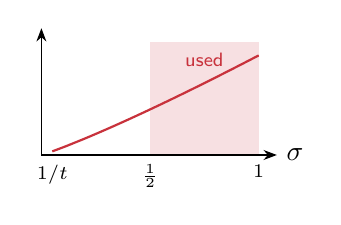
\begin{tikzpicture}[scale=1.15]
  \fill[cRed!15] (1.2,0) rectangle (2.4,1.25);
  \draw[-{Stealth}] (0,0)--(2.6,0) node[right]{$\sigma$};
  \draw[-{Stealth}] (0,0)--(0,1.4);
  \draw[cRed,thick,domain=0.12:2.4,samples=40] plot (\x,{0.5*(\x/2.4)^1.3+0.6*(\x/2.4)});
  \node[below,font=\scriptsize] at (0.12,0) {$1/t$};
  \node[below,font=\scriptsize] at (1.2,0) {$\tfrac12$};
  \node[below,font=\scriptsize] at (2.4,0) {$1$};
  \node[font=\scriptsize,cRed] at (1.8,1.05) {used};
\end{tikzpicture}
\end{minipage}
\begin{keybox}[cRed]
\lab{cRed}{Lemma 2 (curvature).} $\Phi$ is strictly concave in $\eta$ for every $t$, $x$,
$\xi_k$, and $-\nabla_\eta^2\Phi\ge c_R\,I$ on $|\eta|\le R$, with $c_R$ independent of $t$.
\end{keybox}
\lab{cRed}{Consequence.} $\langle\nabla\Phi(\eta)-\nabla\Phi(\eta'),\eta-\eta'\rangle<0$ for
$\eta\ne\eta'$, so $\nabla\Phi$ is injective on all of $\R^{d-1}$. No localization near
critical points is needed.
\end{panel}

\begin{panel}{cTeal}{3}{STEP 3 $\cdot$ DERIVATIVES}
\lab{cTeal}{The problem.} If $\ell_j<\ell_k$, early times magnify $\eta_j$ by
$\sigma^{\ell_j-\ell_k}\gg1$. On the $\eta_j$ axis,
\[
\partial_{\eta_j}^{2N}G(t,0)=(2N)!\binom{1/2}{N}\int_{1/t}^1\sigma^{\ell_k+2N(\ell_j-\ell_k)}d\sigma
\to\infty
\]
as $t\to\infty$, as soon as the exponent is below $-1$.

\lab{cTeal}{The cure.} Measure derivatives in units of $|\eta_j|$: put $w_j=1$ if $j$ is good
and $w_j=|\eta_j|$ if $j$ is bad.
\begin{keybox}[cTeal]
\lab{cTeal}{Lemma 3 (derivatives).} Let $|\alpha|\ge2$ with $\alpha$ supported in $\cO$, and
write $\alpha=\delta_i+\delta_j+\alpha'$ with $i,j\in\cO$ and $\alpha'\ge0$. Then for $t\ge2$,
\[
|\partial_\eta^\alpha\Phi|=|\partial_\eta^\alpha G|\le C_\alpha\prod_{m\ne k}w_m^{-\alpha'_m}.
\]
\end{keybox}
\lab{cTeal}{Why.} With $\mu_m=\sigma^{\ell_m-\ell_k}$ and $y_m=\mu_m\eta_m$, $H=(1+|y|^2)^{1/2}$
behaves like a function homogeneous of degree one, so
$|\partial_\eta^\alpha H|\le C\mu^\alpha H^{1-|\alpha|}$. Each factor $\mu_m/H\le w_m^{-1}$:
for good $m$, $\mu_m\le1\le H$, and for bad $m$, $H\ge\mu_m|\eta_m|$. The two factors for
$i,j$ are paid by
\[
\int_0^1\sigma^{\ell_k}\mu_i\mu_j\,d\sigma\le\tfrac12\int_0^1\big(\sigma^{2\ell_i-\ell_k}+\sigma^{2\ell_j-\ell_k}\big)d\sigma<\infty ,
\]
which is finite exactly because $\kappa_i,\kappa_j>0$.

\remk{cTeal}{Two derivatives in oscillatory directions are free. Each further derivative in a
bad direction costs $1/|\eta_m|$. Non-oscillatory directions are never differentiated.}
\end{panel}

\end{minipage}\hfill
% ================= COLUMN 3 =================
\begin{minipage}[t]{0.322\textwidth}\vspace{0pt}

\begin{panel}{cBlue}{4}{STEP 4 $\cdot$ ZOOM}
\lab{cBlue}{Zoom.} Fix $\xi_k$ and put $\eta=\lambda^{-1/2}\omega$, the stationary phase scale:
\begin{keybox}[cBlue]
\[
J=\lambda^{-\frac{d-1}{2}}\int e^{i\tilde\Phi(\omega)}\,\tilde b(\omega)\,d\omega,\qquad
\tilde\Phi(\omega)=\lambda\,\Phi(\lambda^{-1/2}\omega).
\]
\end{keybox}
\lab{cBlue}{Scaling.} $\partial_\omega^\alpha\tilde\Phi=\lambda^{1-|\alpha|/2}\,\partial_\eta^\alpha\Phi$.
The Hessian is unchanged and higher derivatives shrink. All the decay sits in front, and the
$\omega$ integral only has to be bounded: Theorem 0 with $\lambda=1$.

\begin{center}
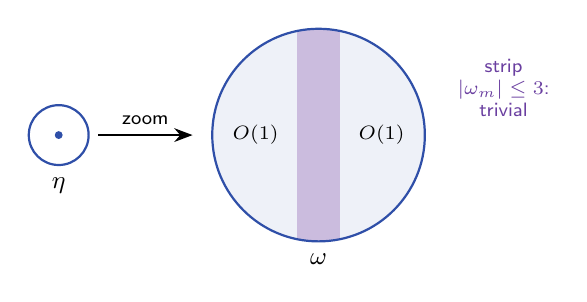
\begin{tikzpicture}[scale=1]
  \draw[thick,cBlue] (0,0) circle (0.38);
  \fill[cBlue] (0,0) circle (0.05);
  \node[below,font=\small] at (0,-0.42) {$\eta$};
  \draw[-{Stealth},thick] (0.5,0)--(1.7,0) node[midway,above,font=\scriptsize]{zoom};
  \begin{scope}[shift={(3.3,0)}]
    \begin{scope}
      \clip (0,0) circle (1.35);
      \fill[cBlue!8] (-1.4,-1.4) rectangle (1.4,1.4);
      \fill[cPurple!35] (-0.27,-1.4) rectangle (0.27,1.4);
    \end{scope}
    \draw[thick,cBlue] (0,0) circle (1.35);
    \node[font=\scriptsize] at (-0.8,0) {$O(1)$};
    \node[font=\scriptsize] at (0.8,0) {$O(1)$};
    \node[below,font=\small] at (0,-1.38) {$\omega$};
    \node[font=\scriptsize,cPurple,align=center] at (2.35,0.6) {strip\\$|\omega_m|\le3$:\\trivial};
  \end{scope}
\end{tikzpicture}
\end{center}

\lab{cBlue}{What one $\omega_j$ derivative costs.}

{\small
\begin{tabular}{@{}p{3.6cm}p{3.5cm}l@{}}
\textbf{falls on} & \textbf{cost} & \textbf{bounded when}\\\hline
cutoff $\tilde\chi$ & $t^{-\kappa_j/2}|\xi_k|^{1/2}$ & $j\in\cO$\\
$\rho_k$, $(1+|\eta|^2)^{-1/2}$ & $\lambda^{-1/2}$ & always\\
phase, bad $m$ (Lemma 3) & $|\omega_m|^{-1}$ & $|\omega_m|\ge1$\\
\end{tabular}}

\remk{cBlue}{In $\xi$: a unit cell in $\omega_j$ has width $t^{-\kappa_j/2}|\xi_k|^{1/2}$ in
$\xi_j$, while $\chi$ varies on scale $1$.}
\end{panel}

\begin{panel}{cPurple}{5}{STEP 5 $\cdot$ STRIPS}
\lab{cPurple}{Strip cutoffs.} Take $\vartheta\in C_0^\infty(\R)$ with $\vartheta=1$ on $[-2,2]$
and $\vartheta=0$ outside $[-3,3]$. For each $m\in\cB$ write
$1=\vartheta(\omega_m)+(1-\vartheta(\omega_m))$ and expand. This gives $2^{|\cB|}$ pieces
$J_S$, where $S\subset\cB$ lists the directions placed in strips.

\lab{cPurple}{Active and frozen.} In $J_S$ the active variables are $A=\cO\setminus S$. The
variables in $S\cup\cT$ are frozen and integrated last.

\lab{cPurple}{1. Theorem 0 in $\omega_A$, with $\lambda=1$.}

{\small
\begin{tabular}{@{}p{2.3cm}p{8.6cm}@{}}
$a_0\ge c^{|A|}$ & Lemma 2 on $|\eta|\le3\sqrt d$; a principal submatrix of a matrix
$\ge cI$ is $\ge cI$\\
injective & Lemma 2: $\tilde\Phi$ is strictly concave in $\omega_A$\\
$\tilde M\le C$ & Lemma 3: $\lambda^{1/2}w_m=\lambda^{1/2}\ge1$ if $m$ good,
$=|\omega_m|\ge1$ off the strips\\
$\tilde N\le C$ & $t^{-\kappa_j/2}|\xi_k|^{1/2}\le\sqrt2$ for $j\in\cO$\\
\end{tabular}}

So the $\omega_A$ integral is at most $C$, uniformly in $x$ and in the frozen variables.

\lab{cPurple}{2. Trivial integration in the frozen variables.}
\begin{itemize}\setlength{\itemsep}{1pt}
  \item $m\in S$: $|\omega_m|\le3$, a factor $6$.
  \item $j\in\cT$: $|\xi_j|\le2$ gives $|\omega_j|\le W_j=2\,t^{\kappa_j/2}|\xi_k|^{-1/2}$,
  a factor $2W_j$.
\end{itemize}
\remk{cPurple}{A strip has width $\lambda^{-1/2}$ in $\eta$: exactly the gain oscillation
would give.}
\end{panel}

\begin{panel}{cMagenta}{6}{STEP 6 $\cdot$ CONCLUSION}
\lab{cMagenta}{Sum the pieces.} Each piece satisfies
\begin{keybox}[cMagenta]
\[
|J_S|\le C\,\lambda^{-\frac{d-1}{2}}\,6^{|S|}\prod_{j\in\cT}2W_j ,
\]
\end{keybox}
and summing over the $2^{|\cB|}$ subsets $S$ gives the main estimate in box B.

\lab{cMagenta}{Uniform in $x$.} $x$ enters $\Phi$ only linearly, and none of $a_0$, $\tilde M$,
$\tilde N$ sees a linear term.

\lab{cMagenta}{Direct versus zoomed.}

{\small
\begin{tabular}{@{}p{3cm}p{4.2cm}p{3.5cm}@{}}
 & \textbf{Theorem 0 in $\eta$} & \textbf{Theorem 0 in $\omega$}\\\hline
amplitude $N$ & $\le C\,t^{d(\ell_k-\ell_{\min})}$ & $\le C$\\
phase $M$ & not uniform in $t$ & $\le C$ off strips\\
\end{tabular}}
\end{panel}

\begin{panel}{cSlate}{$\leftrightarrow$}{CHANGES OF VARIABLES}
{\small
\begin{tabular}{@{}p{3.3cm}p{6.6cm}c@{}}
\textbf{substitution} & \textbf{job} & \textbf{step}\\\hline
$x\to A_tx$ & linear term becomes linear in $\eta$; allowed since the bound is uniform in $x$ & 1\\
$s=\sigma t$ & pulls the large factor $\lambda$ out of the phase & 1\\
$\xi\to(\xi_k,\eta)$ & outer $\xi_k$ integral, inner $\eta$ integral & 1\\
$u=D^{1/2}w$ & Hessian form ready for Cauchy--Schwarz & 2\\
$y_j=\sigma^{\ell_j-\ell_k}\eta_j$ & derivatives of $H$ via $\langle y\rangle$ & 3\\
$\eta=\lambda^{-1/2}\omega$ & decay in front, derivatives at scale $\lambda^{-1/2}$ & 4\\
\end{tabular}}

\remk{cSlate}{Combined: $\xi_j=\pm\,t^{-\kappa_j/2}|\xi_k|^{1/2}\,\omega_j$ for $j\ne k$.}
\end{panel}

\begin{panel}{cGold}{D}{WHERE THE GAIN COMES FROM}
In direction $j$, the support of the amplitude has width $W_j\approx t^{\kappa_j/2}|\xi_k|^{-1/2}$
measured in stationary phase cells.

\begin{center}
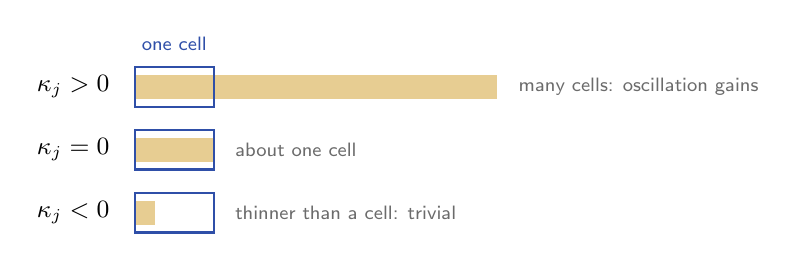
\begin{tikzpicture}[x=1cm,y=1cm]
  \foreach \y/\w/\lbl/\txt in {1.6/4.6/{$\kappa_j>0$}/{many cells: oscillation gains},
                               0.8/1.0/{$\kappa_j=0$}/{about one cell},
                               0/0.25/{$\kappa_j<0$}/{thinner than a cell: trivial}}{
    \node[anchor=east,font=\small] at (-0.2,\y) {\lbl};
    \fill[cGold!45] (0,\y-0.15) rectangle (\w,\y+0.15);
    \draw[cBlue,thick] (0,\y-0.25) rectangle (1,\y+0.25);
    \node[anchor=west,font=\scriptsize,cGray] at ({max(\w,1)+0.15},\y) {\txt};}
  \node[font=\scriptsize,cBlue] at (0.5,2.15) {one cell};
\end{tikzpicture}
\end{center}

\lab{cGold}{$\kappa_j>0$:} the amplitude is smooth on each cell, so oscillation gives
$\lambda^{-1/2}$.\\
\lab{cGold}{$\kappa_j\le0$:} the support is at most about one cell wide, up to
$|\xi_k|^{-1/2}$, so trivial integration already gives the cell's width.
\end{panel}

\end{minipage}

\vspace{2mm}
% ================= SIX MOVES =================
\begin{panel}{cNavy}{\scalebox{1.4}{$\star$}}{THE WHOLE PROOF IN SIX MOVES}
\centering
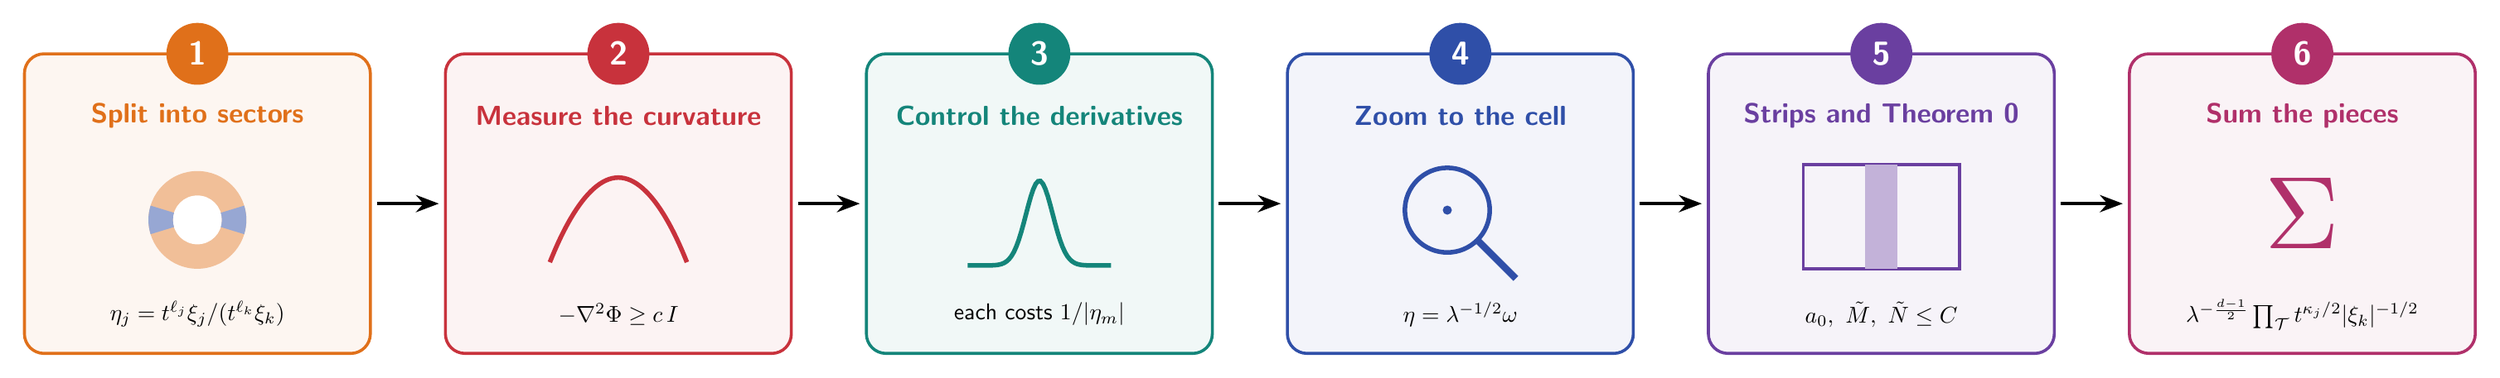
\begin{tikzpicture}[x=1cm,y=1cm]
  \foreach \i/\c/\t/\cap [count=\n from 0] in {
      1/cOrange/{Split into sectors}/{$\eta_j=t^{\ell_j}\xi_j/(t^{\ell_k}\xi_k)$},
      2/cRed/{Measure the curvature}/{$-\nabla^2\Phi\ge c\,I$},
      3/cTeal/{Control the derivatives}/{each costs $1/|\eta_m|$},
      4/cBlue/{Zoom to the cell}/{$\eta=\lambda^{-1/2}\omega$},
      5/cPurple/{Strips and Theorem 0}/{$a_0,\ \tilde M,\ \tilde N\le C$},
      6/cMagenta/{Sum the pieces}/{$\lambda^{-\frac{d-1}{2}}\prod_{\cT}t^{\kappa_j/2}|\xi_k|^{-1/2}$}}{
    \pgfmathsetmacro{\x}{\n*6.45}
    \draw[rounded corners=3mm,line width=1.3pt,draw=\c,fill=\c!6] (\x,0) rectangle ++(5.3,4.6);
    \node[circle,fill=\c,text=white,font=\bfseries\Large,minimum size=0.95cm] at (\x+2.65,4.6) {\i};
    \node[text width=4.9cm,align=center,font=\bfseries\large,text=\c] at (\x+2.65,3.65) {\t};
    \node[font=\normalsize] at (\x+2.65,0.6) {\mbox{\cap}};
    \ifnum\n<5 \draw[-{Stealth[length=3.5mm]},line width=1.6pt] (\x+5.4,2.3)--(\x+6.35,2.3); \fi
  }
  % icons
  \begin{scope}[shift={(2.65,2.05)},scale=0.75]
    \fill[cOrange!45] (0,0) circle (1); \fill[white] (0,0) circle (0.5);
    \foreach \a in {0,180}{\fill[cBlue!50] (\a-17:0.5) arc[start angle=\a-17,end angle=\a+17,radius=0.5]
      -- (\a+17:1) arc[start angle=\a+17,end angle=\a-17,radius=1] -- cycle;}
  \end{scope}
  \draw[cRed,line width=2pt] (6.45+1.6,1.4) parabola bend (6.45+2.65,2.7) (6.45+3.7,1.4);
  \draw[cTeal,line width=2pt,domain=-1.1:1.1,samples=60] plot ({12.9+2.65+\x},{1.35+1.3*exp(-12*\x*\x)});
  \begin{scope}[shift={(19.35+2.45,2.2)}]
    \draw[cBlue,line width=2pt] (0,0) circle (0.65);
    \draw[cBlue,line width=3pt] (0.46,-0.46)--(1.05,-1.05);
    \fill[cBlue] (0,0) circle (0.07);
  \end{scope}
  \begin{scope}[shift={(25.8+2.65,2.1)}]
    \draw[cPurple,line width=1.2pt] (-1.2,-0.8) rectangle (1.2,0.8);
    \fill[cPurple!40] (-0.25,-0.8) rectangle (0.25,0.8);
  \end{scope}
  \node[cMagenta,scale=4.5] at (32.25+2.65,2.15) {$\Sigma$};
\end{tikzpicture}
\end{panel}

% ================= STAR =================
\begin{tcolorbox}[enhanced,colback=cGold!8,colframe=cGold!80,boxrule=1.5pt,arc=3mm,
  left=4mm,right=4mm,top=3mm,bottom=3mm,before skip=0pt]
\begin{minipage}[c]{0.07\linewidth}\centering
\tikz\node[star,star points=5,star point ratio=2.3,fill=cGold,minimum size=1.8cm,inner sep=0pt]{};
\end{minipage}\hfill
\begin{minipage}[c]{0.9\linewidth}\centering\Large\itshape
After zooming to the stationary phase scale $\lambda^{-1/2}$, the condition
\textbf{\color{cBlue}$2\ell_j-\ell_k+1>0$ keeps the amplitude smooth on each cell}.\\
Where it fails, \textbf{\color{cRed}the support is already thinner than one cell}, so that
direction needs no oscillation.
\end{minipage}
\end{tcolorbox}

\end{document}
